%!TEX encoding = UTF-8 Unicode

\section{ウェブインタフェースを介したHPCシステム利用環境}

\subsection{緒言}
前章では,本研究の関連研究について述べた.本章では,ウェブインタフェースを介したHPCシステム利用環境の提案手法について説明し,その実装を行う.はじめに,提案手法の概要を説明する.その後,実装の概要,具体的な実装の手順について説明する.\par

\subsection{提案手法}
本研究の目的は,従来のウェブインタフェースを以下の2つの機能に分離することである.1つは,HPC利用環境をウェブインタフェースに提供する機能 (ウェブ機能)である.もう1つは,ジョブスケジューラ間の差異を抽象化する機能 (スケジューラ抽象化機能)である.この機能の分離により,それぞれの機能を独立に保守管理できる構成を実現する.このために,本研究ではウェブ機能からは統一的にシステムを利用し,スケジューラ抽象化機能でシステム間の差異を埋める構成の利用環境を提案する.\par
この提案手法の模式図を図\ref{fig6}に示す.ウェブ機能では,ユーザはウェブ機能のみとやり取りを行い,ユーザ情報を管理する外部の認証用ディレクトリを用いて安全にHPCシステムを利用することができる.スケジューラ抽象化では,ウェブ機能から得られた様々なジョブスケジューラに対する要求をスケジューラ抽象化機能が受け取り,処理を行う.この実現のためには,ウェブ機能とスケジューラ抽象化機能を連携させる必要があることから,両者間に求められる情報のやり取りを整理し,適切な実装方法を検討する.\par

\begin{figure}[tb]
    \centering
    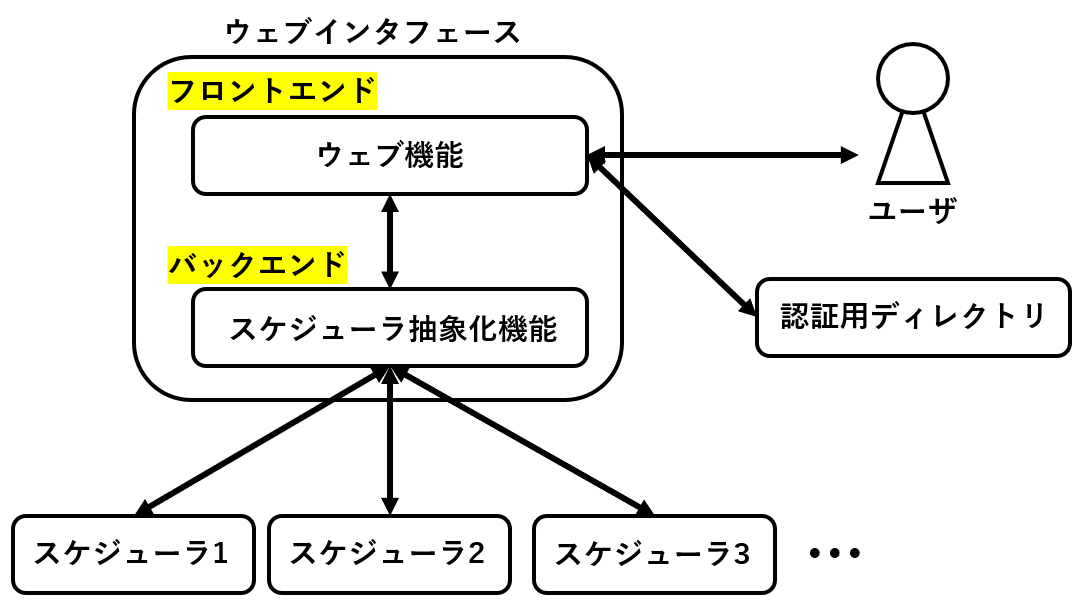
\includegraphics[width=120mm]{./fig/proposed_method.png}
    \caption{提案手法の模式図}
    \label{fig6}
\end{figure}

\subsection{実装}
\subsubsection{実装の概要}
ウェブ機能とスケジューラ抽象化機能をそれぞれ独立に実装し,連携させることでウェブインタフェースを介して様々なシステムを統一的に利用できる環境を実現する.そのために,ウェブ機能の基盤としてOODを利用する.さらに,スケジューラ抽象化機能の基盤としてPSI/J\cite{cite5}と呼ばれるPythonライブラリを利用する.PSI/Jは複数のジョブスケジューラを統一的に取り扱うことを可能とするライブラリである.両者を組み合わせることで提案手法の実装を行う.\par
本研究では,東北大学のスーパーコンピュータ「AOBA」\cite{aoba}で運用されているジョブスケジューラ (NEC Network QueuingSystem V, NQSV) \cite{nqsv_scheduler}がOODに対応していないという事実に着目して,NQSVをスケジューラ抽象化機能側に実装することと,それをウェブ機能側から利用できることを検証する.実装環境として,OOD用のホストサーバとスーパーコンピュータAOBAを模したHPCクラスタ (疑似AOBAクラスタ)を考える.疑似AOBAクラスタの模式図を図\ref{fig7}に示す.OOD用のホストサーバでは,OODの動作が保証されているUbuntu20.04 LSTをOSとして用いる.疑似AOBAクラスタは,マスターノードと二つのワーカーノードから構成される小規模なクラスタであり,AOBAと同様にNQSVをジョブスケジューラとして配備する.疑似AOBAクラスタではNQSVの動作確認が行われているCentOS7を用いる\cite{nqsv_introduction}.本研究の実装では,公式が推奨しているLDAPサーバを用いた「DexとのOpenIDコネクト」を利用して認証を行う\cite{cite7}\cite{cite8}.OpenIDコネクトとはユーザ認証用のプロトコルのことを指す.また,DexとはOpenIDコネクト認証プロバイダーのことを指す.LDAPとは,ユーザIDやパスワードの管理を行うディレクトリサービスの維持およびアクセスを行うプロトコルである.また,LDAPサーバとは,LDAPに基づいてディレクトリサービスを提供するサーバのことである.\par

\begin{figure}[tb]
    \centering
    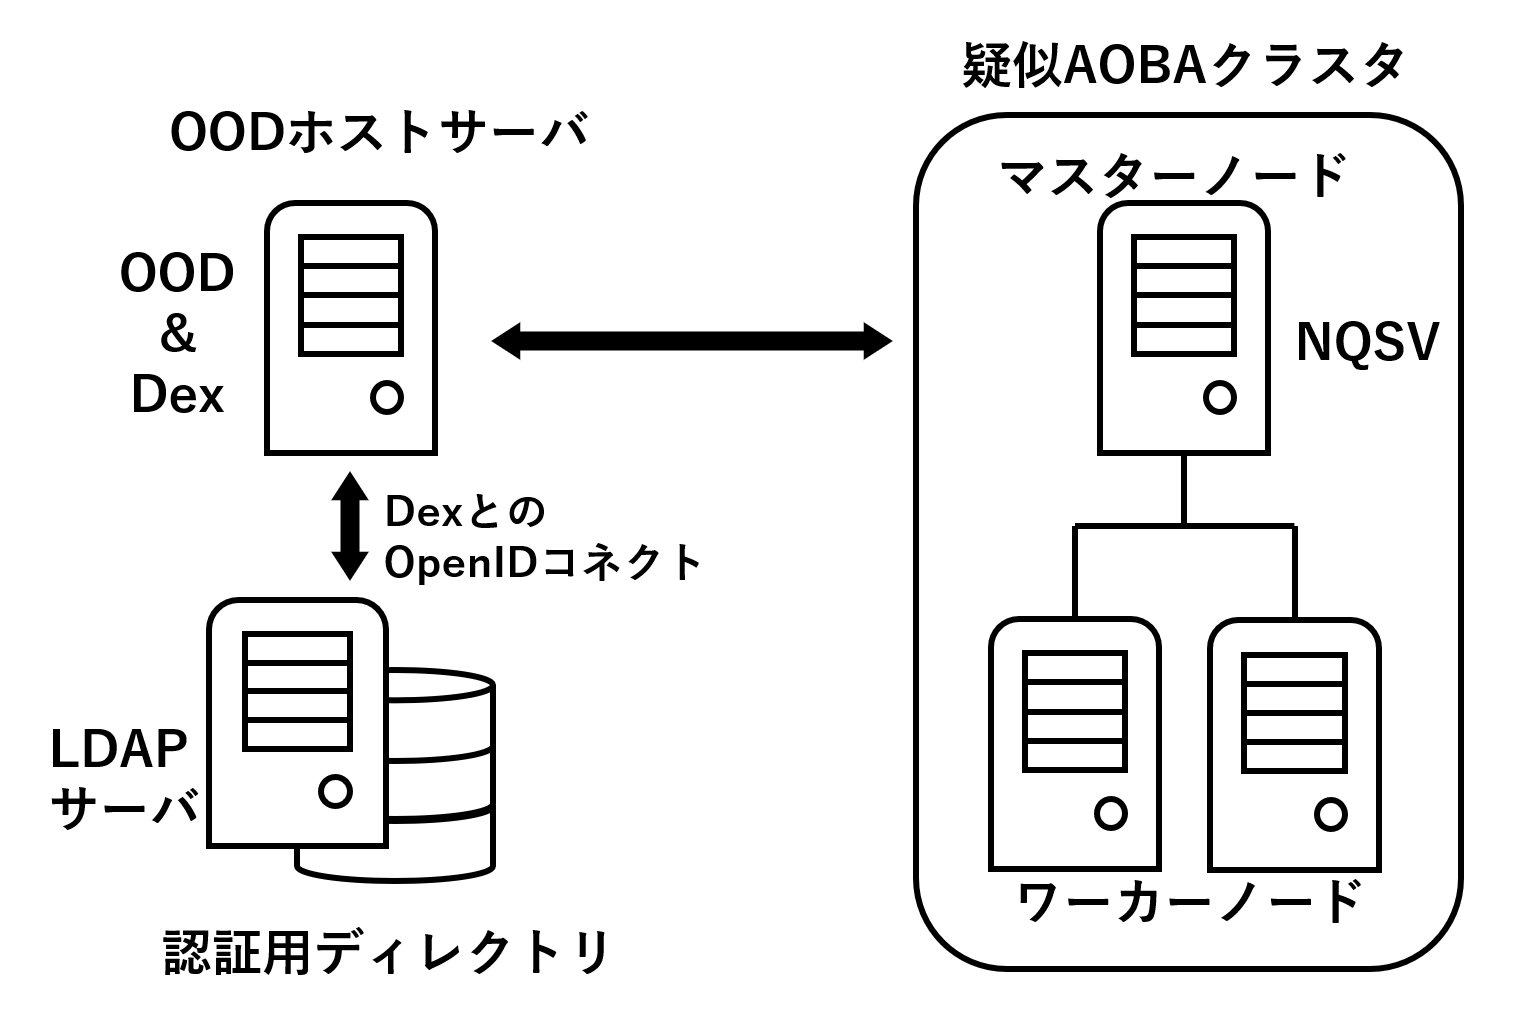
\includegraphics[width=120mm]{./fig/environment.png}
    \caption{実装環境}
    \label{fig7}
\end{figure}


\subsubsection{スケジューラ抽象化機能とNQSVの連携}
スケジューラ抽象化機能とNQSVの連携を考える.スケジューラ抽象化機能の基盤であるPSI/Jは,ジョブの情報を格納するJobクラスとジョブの投入や削除などのメソッドをジョブスケジューラごとに再定義しているJobExecutorクラスにより構成されている.本研究では新たにNQSV用のJobExecutorクラスを作成し,ジョブの投入,削除,及びジョブの状態確認を行うための3つのメソッドを実装する.\par

はじめに,ジョブの投入を行うメソッドを実装する.実装内容をコード\ref{submit}に示す.generate\_submit\_scriptメソッドでは,Jobクラスのオブジェクトであるjob,ジョブ実行に関する情報が格納されたcontext,ジョブスクリプトが書き込まれるファイルオブジェクトであるsubmit\_fileを引数に持ち,generatorオブジェクトのgenerate\_submit\_scriptメソッドを用いて投入するジョブスクリプトファイルの作成を行う.また,get\_submit\_commandでは,投入するジョブスクリプトファイルの絶対パスを用いて,ジョブ投入用のコマンドを作成する.さらに,job\_id\_from\_submit\_outputメソッドでは,引数outにジョブ投入時の標準出力が格納されており,ここからジョブIDを抽出している.NQSVのジョブ投入時の標準出力は「Request ジョブID.NQSVホスト名 submitted to queue: キュー名」である.そのため,ジョブIDを正規表現を用いて抽出し,返り値として出力する.\par

\begin{lstlisting}[caption=ジョブの投入メソッド, label=submit]
class NQSVJobExecutor(BatchSchedulerExecutor):
    def generate_submit_script(self, job: Job, 
                context: Dict[str, object], submit_file: TextIO) -> None:
        self.generator.generate_submit_script(job, context, submit_file)

    def get_submit_command(self, job: Job, submit_file_path: Path)
                                                             -> List[str]:
        return ['qsub', str(submit_file_path.absolute())]

    def job_id_from_submit_output(self, out: str) -> str:
        self.submit_flag = True
        s = out.strip().split()[1]
        out = ""
        match = re.search(r'\b(\d+)\b', s)
        out = match.group() if match else None
        return out
\end{lstlisting}

続いて,ジョブの削除を行うメソッドを実装する.実装内容をコード\ref{cancel}に示す.get\_cancel\_commandメソッドでは,引数であるジョブIDが格納されたnative\_idを用いてジョブ削除用のコマンドを作成する.\par

\begin{lstlisting}[caption=ジョブの削除メソッド, label=cancel]
class NQSVJobExecutor(BatchSchedulerExecutor):    
    def get_cancel_command(self, native_id: str)-> List[str]:
        self.cancel_flag = True
        return ['qdel', native_id]
\end{lstlisting}

最後に,ジョブの状態確認を行うメソッドを実装する.PSI/Jで用いられてるジョブの状態名を表\ref{PSIJstatus}に示す.\par

\begin{table}[tb]
    \centering
    \caption{PSI/Jで用いられているジョブの状態名}
    \begin{tabular}{|l|l|}
    \hline
    状態名       & 説明                  \\ \hline
    NEW       & ジョブがジョブキュー投入前である状態     \\ \hline
    ACTIVE    & ジョブが実行中であるという状態     \\ \hline
    QUEUED    & ジョブがジョブキュー内で待機中である状態 \\ \hline
    COMPLETED & ジョブが実行完了した状態        \\ \hline
    CANCELED  & ジョブが削除された状態         \\ \hline
    FAILED    & ジョブの投入が失敗した状態       \\ \hline
    \end{tabular}
    \label{PSIJstatus}
\end{table}

PSI/Jが対応している他のジョブスケジューラ (Slurm\cite{Slurm},PBS Pro\cite{PBS_Pro},LSF\cite{LSF},Flux\cite{Flux},Cobalt\cite{Cobalt})は,ジョブの終了後にCOMPLETED,CANCELED,及びFAILEDのいずれかの状態であることをジョブの状態を確認するコマンドの出力結果から確認できる.しかし,NQSVではジョブの終了後にCOMPLETED,CANCELED,FAILEDの状態を確認できないという仕様上の違いがある.そのため,NQSVに対応するためには,ジョブの投入,ジョブの削除,および待機中のジョブの存在確認に基づいてジョブの状態をPSI/J側で把握する必要がある.図\ref{state_change_diagram}にはNQSVに対応した場合のジョブの状態遷移図を示す.ジョブが新規作成された瞬間は,ジョブの状態はNEW状態となる.ジョブの投入を行うqstatコマンドが正常に実行されると,ジョブがジョブキュー内に投入されQUEUED状態となる.その後,ジョブの実行が始まるとACTIVE状態に遷移する.NQSVでは,qstatコマンドの出力結果によりQUEUED状態とACTIVE状態を判別することができる.一方,NEW,QUEUED,またはACTIVE状態において,「ジョブキュー内にジョブが存在しない」かつ「ジョブの削除を行うqdelコマンドが実行されている」場合は,ジョブの状態をCANCELED状態に遷移させる.また,「ジョブキュー内にジョブが存在しない」かつ「ジョブの削除を行うqdelコマンドが実行されていない」場合は,ジョブの状態をCOMPLETED状態に遷移させる.また,NEW状態において,ジョブの投入を行うqsubコマンドが失敗した場合はジョブの状態をFAILED状態に遷移させる.\par
具体的な実装をコード\ref{get_status_now}に示す.NQSVJobExecutorクラス内で定義されているget\_status\_nowメソッドはJobクラスのインスタンスを引数にとり,ジョブの状態を保持するJobStatusクラスを返り値に持つ (30行目).引数として受け取ったJobクラスのインスタンス変数job.native\_idからジョブのIDを抽出し,string型変数native\_idsに代入する (31行目).そして,qsubコマンドとそのオプションを用いた「qstat -F rid,stt -n -l native\_ids」コマンドを実行して,ジョブのIDとジョブの状態を取得する (32~34行目)\cite{nqsv_reference}.コマンドの出力は行ごとにList型変数のlinesに代入し,中身をforループで走査する (36~38行目).指定したIDのジョブがジョブキューにない場合は,ジョブのIDとジョブの状態ではなく「Batch Request: ジョブID does not exist on クラスタのホスト名.」という出力が変数lineに代入されるため,条件文「"does not exist on" in line」が真であれば指定したIDのジョブがジョブキューにないということがわかる.そのため,前述した条件文とcancel時に有効化されるcancel\_flagにより,ジョブキュー内にジョブがなく,ジョブの削除が正常に行われていることがわかるため,ジョブの状態をCANCELED状態に遷移させる (43~51行目).一方,条件文が真であり,cancel\_flagが無効である場合は,ジョブキュー内にジョブがないが,ジョブの削除が行われていないので,ジョブの状態をCOMPLETED状態に遷移させる (53~61行目).また,ジョブの投入時に立つsubmit\_flagが立っていない場合はそもそもジョブの投入が成功していないのでジョブの状態をFAILEDにする (63~71行目).以上の3つの場合分けにおいて,「Batch Request: ジョブID does not exist on クラスタのホスト名.」という出力からジョブIDのみを抽出する.抽出したジョブIDごとにDict型変数rを用意して,JobStatusクラスのジョブの状態情報を代入する.また,前述した3種類の場合分けのいずれにも該当しない場合は,ジョブキュー内にジョブが存在する場合であり,ジョブIDとジョブの状態を変数colsに代入する.ここで出力されているジョブの状態はNQSVによって定められた状態名でありジョブキューに投入され,実行待ちである状態はQUE,ジョブが実行されている状態はRUNなど固有の名称が定められている.これらNQSV独自のジョブ状態名からPSI/Jで用いる各ジョブスケジューラで共通の状態名に変換するために,\_STATE\_MAPと\_get\_stateメソッドを用いる.なお,他のジョブスケジューラではジョブ状態の詳細メッセージが出力される場合があるが,NQSVには詳細メッセージの出力機能がないためmessage変数はNoneとしている.\par
このようにPSI/J自身がジョブの状態を管理することにより,さらに広い範囲のジョブスケジューラに対応することができることから,ジョブスケジューラ抽象化機能の汎用性を高めることができたといえる.\par

\begin{figure}[tb]
    \centering
    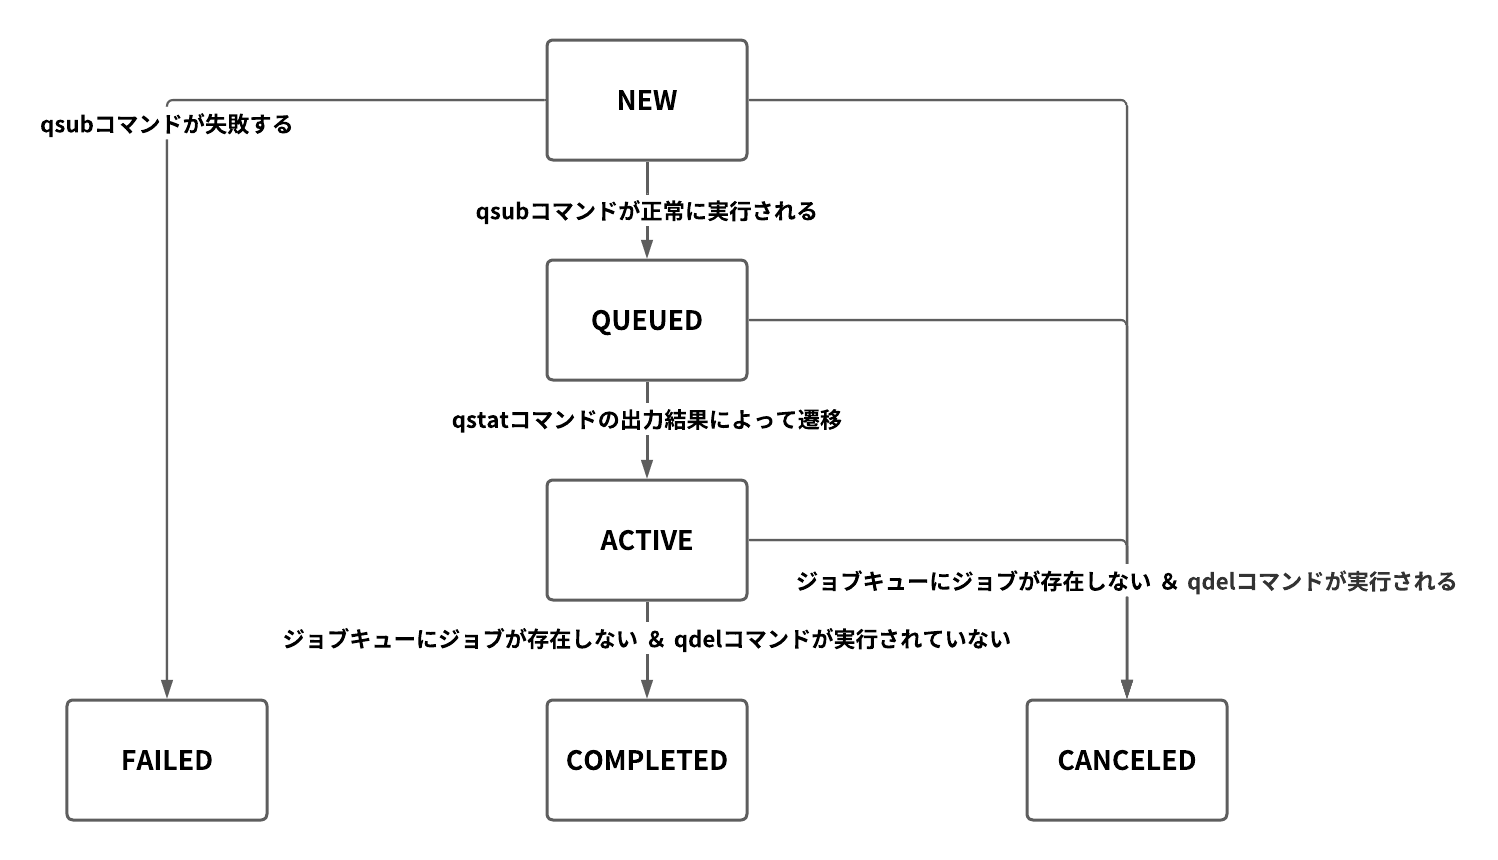
\includegraphics[width=120mm]{./fig/state_change_diagram.png}
    \caption{NQSV対応時のジョブの状態遷移図}
    \label{state_change_diagram}
\end{figure}

\begin{lstlisting}[caption=ジョブの状態取得メソッド, label=get_status_now]
class NQSVJobExecutor(BatchSchedulerExecutor):

    _STATE_MAP = {
        'QUE': JobState.QUEUED,
        'RUN': JobState.ACTIVE,
        'WAT': JobState.QUEUED,
        'HLD': JobState.QUEUED,
        'SUS': JobState.QUEUED,
        'ARI': JobState.QUEUED,
        'TRS': JobState.QUEUED,
        'EXT': JobState.ACTIVE,
        'PRR': JobState.QUEUED,
        'POR': JobState.ACTIVE,
        'MIG': JobState.QUEUED,
        'STG': JobState.QUEUED, 
    }

    def get_status_command(self, native_ids: Collection[str]) -> List[str]:
        return ['qstat', '-F', 'rid,stt', '-n', '-l'] + list(native_ids) 

    def get_status_now(self, job: Job) -> Job.status:
        native_ids = ''.join(str(job.native_id))
        command = ['qstat', '-F', 'rid,stt', '-n', '-l', native_ids]
        out = 
        subprocess.run(command, capture_output=True, text=True).stdout
        r = {}
        lines = iter(out.split('\n'))

        for line in lines:
            if not line:
                continue      

            if(("does not exist on" in line) and self.cancel_flag):
                cols = line.split()
                match = re.search(r'\b(\d+)\b', cols[2])
                native_id = match.group() if match else None
                state = JobState.CANCELED
                r[native_id] = JobStatus(state=state, message=None)
                return r[native_id]
            
            elif(("does not exist on" in line) and not(self.cancel_flag)):
                cols = line.split()
                match = re.search(r'\b(\d+)\b', cols[2])
                native_id = match.group() if match else None
                state = JobState.COMPLETED
                r[native_id] = JobStatus(state=state, message=None)
                return r[native_id]

            elif(not(self.submit_flag)):
                cols = line.split()
                match = re.search(r'\b(\d+)\b', cols[2])
                native_id = match.group() if match else None
                state = JobState.FAILED
                r[native_id] = JobStatus(state=state, message=None)
                return r[native_id]
            
            else:
                cols = line.split()
                match = re.search(r'\b(\d+)\b', cols[0])
                native_id = match.group() if match else None
                native_state = cols[1]
                state = self._get_state(native_state)
                msg = None
                r[native_id] = JobStatus(state=state, message=msg)
                return r[native_id]
    
    def _get_messsage(*args, **kwargs):  
        return None
    
    def _get_state(self, state: str) -> JobState: 
        assert state in NQSVJobExecutor._STATE_MAP
        return NQSVJobExecutor._STATE_MAP[state]
\end{lstlisting}



\subsubsection{ウェブ機能とスケジューラ抽象化機能との連携}
続いて,ウェブ機能を提供するOODからスケジューラ抽象化機能を用いることを考える.実装における問題点として,OODがRubyで実装されていることに対して,PSI/JはPythonで実装されているという点が挙げられる\cite{cite9}\cite{cite10}.そのため,Rubyスクリプト上でPythonライブラリを使用する必要がある.本実装では,PSI/Jを経由する際のオーバヘッドが小さく,単純な実装であるという理由から,PSI/Jを用いたジョブの管理用のPythonスクリプトをシェルを経由してRubyスクリプト上から呼び出す手法を用いる.この実装により,ウェブ機能としてOODを用い,スケジューラ抽象化機能であるPSI/Jを経由して,指定したジョブスケジューラにジョブの投入や削除を行うことができる.また,PSI/Jを仲介することで,OODが未対応であったNQSVでのジョブ管理をOOD上から操作することを実現している.\par
実装をコード\ref{psij_to_ood}に示す.PSI/Jと連携するためのアダプタファイルはOodCore/Job/Adaptersモジュール内で定義され,AdapterスーパークラスのサブクラスとしてPSIJクラスを定義する.コード\ref{config_file}にはOODとPSI/Jを接続するための設定ファイルpsij.ymlの中身を示す.設定ファイルには,OODからログインを行う際のホスト名,選択するAdapter名,PSI/Jで用いるJobExecutorクラス名,ユーザが一般的に使用するコマンドが置かれたバイナリファイルのパスと用いるジョブスケジューラの設定ファイルのパス,ジョブを投入するHPCクラスタのホスト名を設定する.initializeメソッド内では,設定ファイルpsij.ymlから与えられた情報をそれぞれインスタンス変数に代入する (4~13行目).\par
submitメソッドは,引数でジョブスクリプトの内容を文字列として受け取り,投入したジョブのIDを返す.与えらえれたジョブスクリプトは一時的なジョブスクリプト保管用のディレクトリに保存される (16~19行目).その後,scpコマンドを用いて,ユーザのホームディレクトリにPSI/Jを用いたジョブ投入用のPythonスクリプトsubmit\_script.pyが転送される (20~22行目).そして,ジョブ投入先のホストでJobExecutorと投入するジョブのパスを指定してsubmit\_script.pyを実行することで,ジョブを選択したホストに投入する (23~30行目).\par
deleteメソッドは,引数でジョブIDを受け取り,ジョブの削除を行う (33~34行目).submitメソッドと同様に,cpコマンドを用いて,ユーザのホームディレクトリにPSI/Jを用いたジョブ削除用のPythonスクリプトdelete\_script.pyが転送される (35~37行目).そして,ジョブ投入先のホストでJobExecutorと削除するジョブのIDを指定してdelete\_script.pyを実行することで,選択したジョブを削除する (38~43行目).

\begin{lstlisting}[caption=PSI/JとOODの連携, label=psij_to_ood]

class PSIJ < Adapter
  class Batch
    def initialize(cluster: nil, bin: nil, conf: nil, bin_overrides: {}, 
              submit_host: "", strict_host_checking: true, executor: nil)
      @cluster              = cluster && cluster.to_s
      @conf                 = conf    && Pathname.new(conf.to_s)
      @bin                  = Pathname.new(bin.to_s)
      @bin_overrides        = bin_overrides
      @submit_host          = submit_host.to_s
      @strict_host_checking = strict_host_checking
      @executor             = executor
    end

  def submit(script, after: [], afterok: [], afternotok: [], afterany: [])
    job_path = "/Temporary/Path/to/run.sh" 
    file = File.open(job_path, "w")
    file.puts(script.content.to_s)
    file.close
    scp_command = "sshpass -p 'password' scp /Path/to/submit_script.py 
                  username@#{@psij.submit_host}:/Path/to/submit_script.py"
    system(scp_command)
    psij_submit = 
    "python3 /Path/to/submit_script.py" 
                          + " " + @psij.executor + " " + job_path
    ssh_submit = 
    "sshpass -p 'password' 
                  ssh username@#{@psij.submit_host} '#{psij_submit}'"
    o, e, s = Open3.capture3(ssh_submit)
    return o
  end
  
  def delete(id)
    ids = id.to_s
    scp_command = "sshpass -p 'password' scp /Path/to/delete_script.py 
                  username@#{@psij.submit_host}:/Path/to/delete_script.py"
    system(scp_command)
    psij_delete = 
    "python3 /ood_tmp/delete_script.py" + " " + @psij.executor + " " + ids
    ssh_delete = 
    "sshpass -p 'password' 
                  ssh username@#{@psij.submit_host} '#{psij_delete}'"
    system(ssh_delete)
  end

\end{lstlisting}

\begin{lstlisting}[caption=OODとPSI/Jの接続ファイル, label=config_file]
v2:
    metadata:
      title: "PSIJ"
    login:
      host: "host adress"
    job:
      adapter: "psij"
      bin: /path/to/bin
      conf: /path/to/nqsv.conf
      executor: "nqsv"
      submit_host: "submit_host adress"
\end{lstlisting}

\subsection{結言}
本章では,ウェブインタフェースを介したHPCシステム利用環境の提案手法について説明し,その実装を行った.はじめに,提案手法の概要を説明した.本研究では,ウェブインタフェースをウェブ機能とスケジューラ抽象化機能をそれぞれ独立して実装することで,新たなジョブスケジューラに対応する際の保守性に関する問題を解決することを目指す.その後,実装の概要,具体的な実装の手順について説明した.ウェブ機能の基盤としてOOD,スケジューラ抽象化機能の基盤としてPSI/Jを用いる.両者を連携させ,ウェブ機能からスケジューラ抽象化機能を介してNQSVを利用できるように実装を行った.次章では,本章で実装した提案手法の評価を行い,提案手法の実現可能性と有用性を考察する.